\documentclass[twoside]{book}

% Packages required by doxygen
\usepackage{fixltx2e}
\usepackage{calc}
\usepackage{doxygen}
\usepackage[export]{adjustbox} % also loads graphicx
\usepackage{graphicx}
\usepackage[utf8]{inputenc}
\usepackage{makeidx}
\usepackage{multicol}
\usepackage{multirow}
\PassOptionsToPackage{warn}{textcomp}
\usepackage{textcomp}
\usepackage[nointegrals]{wasysym}
\usepackage[table]{xcolor}

% Font selection
\usepackage[T1]{fontenc}
\usepackage[scaled=.90]{helvet}
\usepackage{courier}
\usepackage{amssymb}
\usepackage{sectsty}
\renewcommand{\familydefault}{\sfdefault}
\allsectionsfont{%
  \fontseries{bc}\selectfont%
  \color{darkgray}%
}
\renewcommand{\DoxyLabelFont}{%
  \fontseries{bc}\selectfont%
  \color{darkgray}%
}
\newcommand{\+}{\discretionary{\mbox{\scriptsize$\hookleftarrow$}}{}{}}

% Page & text layout
\usepackage{geometry}
\geometry{%
  a4paper,%
  top=2.5cm,%
  bottom=2.5cm,%
  left=2.5cm,%
  right=2.5cm%
}
\tolerance=750
\hfuzz=15pt
\hbadness=750
\setlength{\emergencystretch}{15pt}
\setlength{\parindent}{0cm}
\setlength{\parskip}{3ex plus 2ex minus 2ex}
\makeatletter
\renewcommand{\paragraph}{%
  \@startsection{paragraph}{4}{0ex}{-1.0ex}{1.0ex}{%
    \normalfont\normalsize\bfseries\SS@parafont%
  }%
}
\renewcommand{\subparagraph}{%
  \@startsection{subparagraph}{5}{0ex}{-1.0ex}{1.0ex}{%
    \normalfont\normalsize\bfseries\SS@subparafont%
  }%
}
\makeatother

% Headers & footers
\usepackage{fancyhdr}
\pagestyle{fancyplain}
\fancyhead[LE]{\fancyplain{}{\bfseries\thepage}}
\fancyhead[CE]{\fancyplain{}{}}
\fancyhead[RE]{\fancyplain{}{\bfseries\leftmark}}
\fancyhead[LO]{\fancyplain{}{\bfseries\rightmark}}
\fancyhead[CO]{\fancyplain{}{}}
\fancyhead[RO]{\fancyplain{}{\bfseries\thepage}}
\fancyfoot[LE]{\fancyplain{}{}}
\fancyfoot[CE]{\fancyplain{}{}}
\fancyfoot[RE]{\fancyplain{}{\bfseries\scriptsize Generated by Doxygen }}
\fancyfoot[LO]{\fancyplain{}{\bfseries\scriptsize Generated by Doxygen }}
\fancyfoot[CO]{\fancyplain{}{}}
\fancyfoot[RO]{\fancyplain{}{}}
\renewcommand{\footrulewidth}{0.4pt}
\renewcommand{\chaptermark}[1]{%
  \markboth{#1}{}%
}
\renewcommand{\sectionmark}[1]{%
  \markright{\thesection\ #1}%
}

% Indices & bibliography
\usepackage{natbib}
\usepackage[titles]{tocloft}
\setcounter{tocdepth}{3}
\setcounter{secnumdepth}{5}
\makeindex

% Hyperlinks (required, but should be loaded last)
\usepackage{ifpdf}
\ifpdf
  \usepackage[pdftex,pagebackref=true]{hyperref}
\else
  \usepackage[ps2pdf,pagebackref=true]{hyperref}
\fi
\hypersetup{%
  colorlinks=true,%
  linkcolor=blue,%
  citecolor=blue,%
  unicode%
}

% Custom commands
\newcommand{\clearemptydoublepage}{%
  \newpage{\pagestyle{empty}\cleardoublepage}%
}

\usepackage{caption}
\captionsetup{labelsep=space,justification=centering,font={bf},singlelinecheck=off,skip=4pt,position=top}

%===== C O N T E N T S =====

\begin{document}

% Titlepage & ToC
\hypersetup{pageanchor=false,
             bookmarksnumbered=true,
             pdfencoding=unicode
            }
\pagenumbering{roman}
\begin{titlepage}
\vspace*{7cm}
\begin{center}%
{\Large Wifi\+Killer }\\
\vspace*{1cm}
{\large Generated by Doxygen 1.8.11}\\
\end{center}
\end{titlepage}
\clearemptydoublepage
\tableofcontents
\clearemptydoublepage
\pagenumbering{arabic}
\hypersetup{pageanchor=true}

%--- Begin generated contents ---
\chapter{Class Index}
\section{Class List}
Here are the classes, structs, unions and interfaces with brief descriptions\+:\begin{DoxyCompactList}
\item\contentsline{section}{\hyperlink{structether__hdr}{ether\+\_\+hdr} }{\pageref{structether__hdr}}{}
\item\contentsline{section}{\hyperlink{structframe__control}{frame\+\_\+control} }{\pageref{structframe__control}}{}
\item\contentsline{section}{\hyperlink{structfstr__s}{fstr\+\_\+s} }{\pageref{structfstr__s}}{}
\item\contentsline{section}{\hyperlink{structip__hdr}{ip\+\_\+hdr} }{\pageref{structip__hdr}}{}
\item\contentsline{section}{\hyperlink{structok__array}{ok\+\_\+array} }{\pageref{structok__array}}{}
\item\contentsline{section}{\hyperlink{structtcp__hdr}{tcp\+\_\+hdr} }{\pageref{structtcp__hdr}}{}
\item\contentsline{section}{\hyperlink{structwlan__hdr}{wlan\+\_\+hdr} }{\pageref{structwlan__hdr}}{}
\end{DoxyCompactList}

\chapter{File Index}
\section{File List}
Here is a list of all documented files with brief descriptions\+:\begin{DoxyCompactList}
\item\contentsline{section}{\hyperlink{cappacket_8c}{cappacket.\+c} }{\pageref{cappacket_8c}}{}
\item\contentsline{section}{{\bfseries cappacket.\+h} }{\pageref{cappacket_8h}}{}
\item\contentsline{section}{{\bfseries config.\+h} }{\pageref{config_8h}}{}
\item\contentsline{section}{{\bfseries fstr.\+h} }{\pageref{fstr_8h}}{}
\item\contentsline{section}{{\bfseries hacking-\/network.\+h} }{\pageref{hacking-network_8h}}{}
\item\contentsline{section}{{\bfseries hacking.\+h} }{\pageref{hacking_8h}}{}
\item\contentsline{section}{{\bfseries monitor.\+h} }{\pageref{monitor_8h}}{}
\item\contentsline{section}{{\bfseries string\+\_\+utilities.\+h} }{\pageref{string__utilities_8h}}{}
\end{DoxyCompactList}

\chapter{Class Documentation}
\hypertarget{structether__hdr}{}\section{ether\+\_\+hdr Struct Reference}
\label{structether__hdr}\index{ether\+\_\+hdr@{ether\+\_\+hdr}}
\subsection*{Public Attributes}
\begin{DoxyCompactItemize}
\item 
unsigned char {\bfseries ether\+\_\+dest\+\_\+addr} \mbox{[}E\+T\+H\+E\+R\+\_\+\+A\+D\+D\+R\+\_\+\+L\+EN\mbox{]}\hypertarget{structether__hdr_a75ac8d938e5b4c8ace0c7989df8ccf96}{}\label{structether__hdr_a75ac8d938e5b4c8ace0c7989df8ccf96}

\item 
unsigned char {\bfseries ether\+\_\+src\+\_\+addr} \mbox{[}E\+T\+H\+E\+R\+\_\+\+A\+D\+D\+R\+\_\+\+L\+EN\mbox{]}\hypertarget{structether__hdr_a28e500aa274f4e0e238daf1111d37864}{}\label{structether__hdr_a28e500aa274f4e0e238daf1111d37864}

\item 
unsigned short {\bfseries ether\+\_\+type}\hypertarget{structether__hdr_aa06fcc3a21680faa65b24c6e6f97832b}{}\label{structether__hdr_aa06fcc3a21680faa65b24c6e6f97832b}

\end{DoxyCompactItemize}


The documentation for this struct was generated from the following file\+:\begin{DoxyCompactItemize}
\item 
hacking-\/network.\+h\end{DoxyCompactItemize}

\hypertarget{structframe__control}{}\section{frame\+\_\+control Struct Reference}
\label{structframe__control}\index{frame\+\_\+control@{frame\+\_\+control}}
\subsection*{Public Attributes}
\begin{DoxyCompactItemize}
\item 
unsigned short {\bfseries protocol}\+:2\hypertarget{structframe__control_a75f4c8f943d360e711acf8e3fbbfbba9}{}\label{structframe__control_a75f4c8f943d360e711acf8e3fbbfbba9}

\item 
unsigned short {\bfseries type}\+:2\hypertarget{structframe__control_afb27db9aa36003679b44cdceaa00ff6a}{}\label{structframe__control_afb27db9aa36003679b44cdceaa00ff6a}

\item 
unsigned short {\bfseries sub\+\_\+type}\+:4\hypertarget{structframe__control_a0cf228b97548bbd1721073b6ce48a1fc}{}\label{structframe__control_a0cf228b97548bbd1721073b6ce48a1fc}

\item 
unsigned short {\bfseries to\+\_\+ds}\+:1\hypertarget{structframe__control_a1db4f7b27647ee5e2882b1fc82b31508}{}\label{structframe__control_a1db4f7b27647ee5e2882b1fc82b31508}

\item 
unsigned short {\bfseries from\+\_\+ds}\+:1\hypertarget{structframe__control_a2b6204224bf81f98f672e90ac9242471}{}\label{structframe__control_a2b6204224bf81f98f672e90ac9242471}

\item 
unsigned short {\bfseries more\+\_\+frag}\+:1\hypertarget{structframe__control_aab6c806b88227e9837fba037087153ac}{}\label{structframe__control_aab6c806b88227e9837fba037087153ac}

\item 
unsigned short {\bfseries retry}\+:1\hypertarget{structframe__control_a0bd8c587c2c09d7b5f88bdb8bad44a3c}{}\label{structframe__control_a0bd8c587c2c09d7b5f88bdb8bad44a3c}

\item 
unsigned short {\bfseries power\+\_\+mgmt}\+:1\hypertarget{structframe__control_a92f169e8b6d17af88fef2b2beb6380fc}{}\label{structframe__control_a92f169e8b6d17af88fef2b2beb6380fc}

\item 
unsigned short {\bfseries more\+\_\+data}\+:1\hypertarget{structframe__control_adb5ce701741169ba4fa77df68a69b065}{}\label{structframe__control_adb5ce701741169ba4fa77df68a69b065}

\item 
unsigned short {\bfseries protected\+\_\+frame}\+:1\hypertarget{structframe__control_ac75f11025ccedefde9276f821cdc8942}{}\label{structframe__control_ac75f11025ccedefde9276f821cdc8942}

\item 
unsigned short {\bfseries order}\+:1\hypertarget{structframe__control_a7d79b0e2031f96da1573d09b4c60447f}{}\label{structframe__control_a7d79b0e2031f96da1573d09b4c60447f}

\end{DoxyCompactItemize}


The documentation for this struct was generated from the following file\+:\begin{DoxyCompactItemize}
\item 
hacking-\/network.\+h\end{DoxyCompactItemize}

\hypertarget{structfstr__s}{}\section{fstr\+\_\+s Struct Reference}
\label{structfstr__s}\index{fstr\+\_\+s@{fstr\+\_\+s}}
\subsection*{Public Attributes}
\begin{DoxyCompactItemize}
\item 
char $\ast$ {\bfseries data}\hypertarget{structfstr__s_adc44dd3a33ce7b32d9b9a85f1a0c2d50}{}\label{structfstr__s_adc44dd3a33ce7b32d9b9a85f1a0c2d50}

\item 
size\+\_\+t {\bfseries start}\hypertarget{structfstr__s_a52c8d6feff8a8245b6eae1c21f6d125e}{}\label{structfstr__s_a52c8d6feff8a8245b6eae1c21f6d125e}

\item 
size\+\_\+t {\bfseries end}\hypertarget{structfstr__s_a5da96a1a85832106ab8fa7a97772ce8b}{}\label{structfstr__s_a5da96a1a85832106ab8fa7a97772ce8b}

\item 
int $\ast$ {\bfseries refs}\hypertarget{structfstr__s_ad22b636b6bfc40a1348ee2fab0110405}{}\label{structfstr__s_ad22b636b6bfc40a1348ee2fab0110405}

\end{DoxyCompactItemize}


The documentation for this struct was generated from the following file\+:\begin{DoxyCompactItemize}
\item 
fstr.\+h\end{DoxyCompactItemize}

\hypertarget{structip__hdr}{}\section{ip\+\_\+hdr Struct Reference}
\label{structip__hdr}\index{ip\+\_\+hdr@{ip\+\_\+hdr}}
\subsection*{Public Attributes}
\begin{DoxyCompactItemize}
\item 
unsigned char {\bfseries ip\+\_\+version\+\_\+and\+\_\+header\+\_\+length}\hypertarget{structip__hdr_ab284c6984e507834968090a46de21f1a}{}\label{structip__hdr_ab284c6984e507834968090a46de21f1a}

\item 
unsigned char {\bfseries ip\+\_\+tos}\hypertarget{structip__hdr_af50662ba23d9f6c2b0d00532e828d39d}{}\label{structip__hdr_af50662ba23d9f6c2b0d00532e828d39d}

\item 
unsigned short {\bfseries ip\+\_\+len}\hypertarget{structip__hdr_ac902256d48b81f3226404c7d32a01569}{}\label{structip__hdr_ac902256d48b81f3226404c7d32a01569}

\item 
unsigned short {\bfseries ip\+\_\+id}\hypertarget{structip__hdr_a4eda327cff29c1dddb471b5a9d07580b}{}\label{structip__hdr_a4eda327cff29c1dddb471b5a9d07580b}

\item 
unsigned short {\bfseries ip\+\_\+frag\+\_\+offset}\hypertarget{structip__hdr_a7c4b79d751553f232eefe6c5d54a3af3}{}\label{structip__hdr_a7c4b79d751553f232eefe6c5d54a3af3}

\item 
unsigned char {\bfseries ip\+\_\+ttl}\hypertarget{structip__hdr_af5bbc5a58545da2185f62dfc171bec7b}{}\label{structip__hdr_af5bbc5a58545da2185f62dfc171bec7b}

\item 
unsigned char {\bfseries ip\+\_\+type}\hypertarget{structip__hdr_a786dba97704c69307d37092b8b0dd880}{}\label{structip__hdr_a786dba97704c69307d37092b8b0dd880}

\item 
unsigned short {\bfseries ip\+\_\+checksum}\hypertarget{structip__hdr_abc1ee3f70a6d9b45823b34db2725b6f6}{}\label{structip__hdr_abc1ee3f70a6d9b45823b34db2725b6f6}

\item 
unsigned int {\bfseries ip\+\_\+src\+\_\+addr}\hypertarget{structip__hdr_adfce267129d461c1d2ac9a1bc67abd89}{}\label{structip__hdr_adfce267129d461c1d2ac9a1bc67abd89}

\item 
unsigned int {\bfseries ip\+\_\+dest\+\_\+addr}\hypertarget{structip__hdr_afacfc2edd2bb2af45b8f505aaf6dea6c}{}\label{structip__hdr_afacfc2edd2bb2af45b8f505aaf6dea6c}

\end{DoxyCompactItemize}


The documentation for this struct was generated from the following file\+:\begin{DoxyCompactItemize}
\item 
hacking-\/network.\+h\end{DoxyCompactItemize}

\hypertarget{structok__array}{}\section{ok\+\_\+array Struct Reference}
\label{structok__array}\index{ok\+\_\+array@{ok\+\_\+array}}
\subsection*{Public Attributes}
\begin{DoxyCompactItemize}
\item 
char $\ast$$\ast$ {\bfseries elements}\hypertarget{structok__array_ae35954941500b16a37e47875bcf2d113}{}\label{structok__array_ae35954941500b16a37e47875bcf2d113}

\item 
char $\ast$ {\bfseries base\+\_\+string}\hypertarget{structok__array_aa6bb78efcd51274d5bcaf946d2d932d3}{}\label{structok__array_aa6bb78efcd51274d5bcaf946d2d932d3}

\item 
int {\bfseries length}\hypertarget{structok__array_a6d1bcc323c770d425d7e8734e6c37a07}{}\label{structok__array_a6d1bcc323c770d425d7e8734e6c37a07}

\end{DoxyCompactItemize}


The documentation for this struct was generated from the following file\+:\begin{DoxyCompactItemize}
\item 
string\+\_\+utilities.\+h\end{DoxyCompactItemize}

\hypertarget{structtcp__hdr}{}\section{tcp\+\_\+hdr Struct Reference}
\label{structtcp__hdr}\index{tcp\+\_\+hdr@{tcp\+\_\+hdr}}
\subsection*{Public Attributes}
\begin{DoxyCompactItemize}
\item 
unsigned short {\bfseries tcp\+\_\+src\+\_\+port}\hypertarget{structtcp__hdr_aa136b16207341d31d6ded12b85b4d2ba}{}\label{structtcp__hdr_aa136b16207341d31d6ded12b85b4d2ba}

\item 
unsigned short {\bfseries tcp\+\_\+dest\+\_\+port}\hypertarget{structtcp__hdr_a90e97bacd4c32851ba0d9b859297affb}{}\label{structtcp__hdr_a90e97bacd4c32851ba0d9b859297affb}

\item 
unsigned int {\bfseries tcp\+\_\+seq}\hypertarget{structtcp__hdr_ab831d1a38bb8ff93bf2acade137a711d}{}\label{structtcp__hdr_ab831d1a38bb8ff93bf2acade137a711d}

\item 
unsigned int {\bfseries tcp\+\_\+ack}\hypertarget{structtcp__hdr_aeaa8bb11cb2f52ec565ebb47f1e412b9}{}\label{structtcp__hdr_aeaa8bb11cb2f52ec565ebb47f1e412b9}

\item 
unsigned char {\bfseries reserved}\+:4\hypertarget{structtcp__hdr_ad791ec1d361c5ecc47c04cef06765a55}{}\label{structtcp__hdr_ad791ec1d361c5ecc47c04cef06765a55}

\item 
unsigned char {\bfseries tcp\+\_\+offset}\+:4\hypertarget{structtcp__hdr_a0caf29f03eabb0c93ec782a5f598fd94}{}\label{structtcp__hdr_a0caf29f03eabb0c93ec782a5f598fd94}

\item 
unsigned char {\bfseries tcp\+\_\+flags}\hypertarget{structtcp__hdr_a57f5cce6d80adf9068ce5dd24f087440}{}\label{structtcp__hdr_a57f5cce6d80adf9068ce5dd24f087440}

\item 
unsigned short {\bfseries tcp\+\_\+window}\hypertarget{structtcp__hdr_a32dc94859ff3068a5430b2da55a88371}{}\label{structtcp__hdr_a32dc94859ff3068a5430b2da55a88371}

\item 
unsigned short {\bfseries tcp\+\_\+checksum}\hypertarget{structtcp__hdr_a977ff214ee61b33b707a8b2105f1f8e6}{}\label{structtcp__hdr_a977ff214ee61b33b707a8b2105f1f8e6}

\item 
unsigned short {\bfseries tcp\+\_\+urgent}\hypertarget{structtcp__hdr_a27c6d010ef1f223788a7a7a0f5a67be0}{}\label{structtcp__hdr_a27c6d010ef1f223788a7a7a0f5a67be0}

\end{DoxyCompactItemize}


The documentation for this struct was generated from the following file\+:\begin{DoxyCompactItemize}
\item 
hacking-\/network.\+h\end{DoxyCompactItemize}

\hypertarget{structwlan__hdr}{}\section{wlan\+\_\+hdr Struct Reference}
\label{structwlan__hdr}\index{wlan\+\_\+hdr@{wlan\+\_\+hdr}}
\subsection*{Public Attributes}
\begin{DoxyCompactItemize}
\item 
unsigned short {\bfseries framecon}\hypertarget{structwlan__hdr_a246c63b452dccce486a8e9169352f544}{}\label{structwlan__hdr_a246c63b452dccce486a8e9169352f544}

\item 
unsigned short {\bfseries duration}\hypertarget{structwlan__hdr_a200a05f9ec5516916c4045c94f14c9ae}{}\label{structwlan__hdr_a200a05f9ec5516916c4045c94f14c9ae}

\item 
unsigned char {\bfseries ra} \mbox{[}E\+T\+H\+E\+R\+\_\+\+A\+D\+D\+R\+\_\+\+L\+EN\mbox{]}\hypertarget{structwlan__hdr_afc9d3d64050ee51b75e0c7366d394f66}{}\label{structwlan__hdr_afc9d3d64050ee51b75e0c7366d394f66}

\item 
unsigned char {\bfseries ta} \mbox{[}E\+T\+H\+E\+R\+\_\+\+A\+D\+D\+R\+\_\+\+L\+EN\mbox{]}\hypertarget{structwlan__hdr_ae2539d3f620fdd7b2919c4085604c409}{}\label{structwlan__hdr_ae2539d3f620fdd7b2919c4085604c409}

\item 
unsigned char {\bfseries da} \mbox{[}E\+T\+H\+E\+R\+\_\+\+A\+D\+D\+R\+\_\+\+L\+EN\mbox{]}\hypertarget{structwlan__hdr_a06071d966c04d8c2af4e03076afcb385}{}\label{structwlan__hdr_a06071d966c04d8c2af4e03076afcb385}

\item 
unsigned short {\bfseries seq\+\_\+control}\hypertarget{structwlan__hdr_ad88bc1e7729d9924bbbb49806a868fe7}{}\label{structwlan__hdr_ad88bc1e7729d9924bbbb49806a868fe7}

\item 
unsigned char {\bfseries sa} \mbox{[}E\+T\+H\+E\+R\+\_\+\+A\+D\+D\+R\+\_\+\+L\+EN\mbox{]}\hypertarget{structwlan__hdr_a92e14713106ce270e88a694473103dcb}{}\label{structwlan__hdr_a92e14713106ce270e88a694473103dcb}

\end{DoxyCompactItemize}


The documentation for this struct was generated from the following file\+:\begin{DoxyCompactItemize}
\item 
hacking-\/network.\+h\end{DoxyCompactItemize}

\chapter{File Documentation}
\hypertarget{cappacket_8c}{}\section{cappacket.\+c File Reference}
\label{cappacket_8c}\index{cappacket.\+c@{cappacket.\+c}}
{\ttfamily \#include $<$unistd.\+h$>$}\\*
{\ttfamily \#include $<$pcap.\+h$>$}\\*
{\ttfamily \#include $<$stdlib.\+h$>$}\\*
{\ttfamily \#include $<$sys/socket.\+h$>$}\\*
{\ttfamily \#include $<$netinet/in.\+h$>$}\\*
{\ttfamily \#include $<$arpa/inet.\+h$>$}\\*
{\ttfamily \#include \char`\"{}hacking.\+h\char`\"{}}\\*
{\ttfamily \#include \char`\"{}hacking-\/network.\+h\char`\"{}}\\*
Include dependency graph for cappacket.\+c\+:
\nopagebreak
\begin{figure}[H]
\begin{center}
\leavevmode
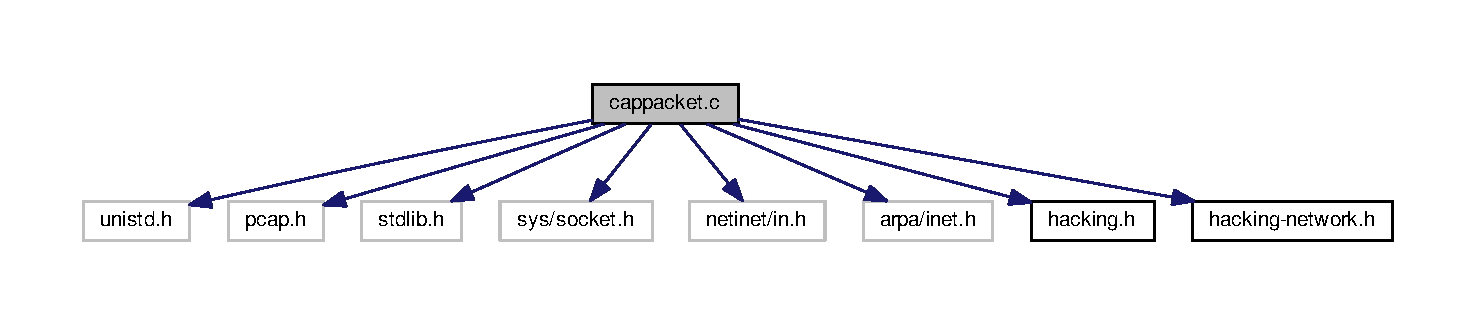
\includegraphics[width=350pt]{cappacket_8c__incl}
\end{center}
\end{figure}
\subsection*{Functions}
\begin{DoxyCompactItemize}
\item 
void \hyperlink{cappacket_8c_a8b147210f8115cd259b966fb68899f04}{parse\+\_\+wlanframe} (u\+\_\+char $\ast$user\+\_\+args, const struct pcap\+\_\+pkthdr $\ast$cap\+\_\+header, const u\+\_\+char $\ast$packet)
\begin{DoxyCompactList}\small\item\em callback function for pcap\+\_\+loop. \end{DoxyCompactList}\end{DoxyCompactItemize}


\subsection{Function Documentation}
\index{cappacket.\+c@{cappacket.\+c}!parse\+\_\+wlanframe@{parse\+\_\+wlanframe}}
\index{parse\+\_\+wlanframe@{parse\+\_\+wlanframe}!cappacket.\+c@{cappacket.\+c}}
\subsubsection[{\texorpdfstring{parse\+\_\+wlanframe(u\+\_\+char $\ast$user\+\_\+args, const struct pcap\+\_\+pkthdr $\ast$cap\+\_\+header, const u\+\_\+char $\ast$packet)}{parse_wlanframe(u_char *user_args, const struct pcap_pkthdr *cap_header, const u_char *packet)}}]{\setlength{\rightskip}{0pt plus 5cm}void parse\+\_\+wlanframe (
\begin{DoxyParamCaption}
\item[{u\+\_\+char $\ast$}]{user\+\_\+args, }
\item[{const struct pcap\+\_\+pkthdr $\ast$}]{cap\+\_\+header, }
\item[{const u\+\_\+char $\ast$}]{packet}
\end{DoxyParamCaption}
)}\hypertarget{cappacket_8c_a8b147210f8115cd259b966fb68899f04}{}\label{cappacket_8c_a8b147210f8115cd259b966fb68899f04}


callback function for pcap\+\_\+loop. 


\begin{DoxyParams}{Parameters}
{\em user\+\_\+args} & custom user arguments from the pcap\+\_\+loop function. \\
\hline
{\em cap\+\_\+header} & libpcap metadata header about the packet. \\
\hline
{\em packet} & pointer to the captured packet \\
\hline
\end{DoxyParams}

%--- End generated contents ---

% Index
\backmatter
\newpage
\phantomsection
\clearemptydoublepage
\addcontentsline{toc}{chapter}{Index}
\printindex

\end{document}
